\section{Durchführung}
\label{sec:Durchführung}
Zunächst soll die Zeitkonstante eines RC-Gliedes durch die Beobachtung und Auswertung
der Spannung am Kondensator bestimmt werden. Dafür wird die in \ref{fig:Schaltung_4a}
gezeigte Schaltung verwendet. An das RC-Glied wird dabei mit einem Multimeter eine
Rechteckspannung angelegt. Die Spannung $U_{\text{C}}$ am Kondensator wird abgegriffen und auf dem
Oszilloskop so dargestellt, dass eine abfallende Flanke möglichst genau zu erkennen ist.
Danach wird ein Bild des Graphen erstellt, aus dem Wertepaare für die Spannung $U$
und die Zeit $t$ abgelesen werden können.

\begin{figure}
  \centering
  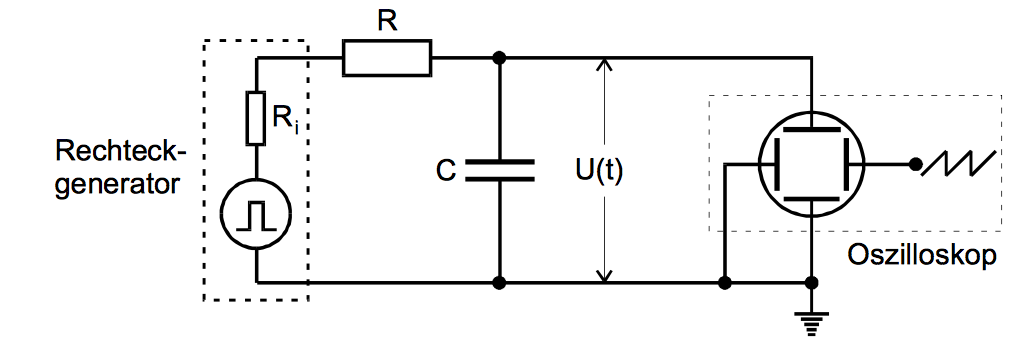
\includegraphics[width=300pt]{data/4a_schaltung.png}
  \caption{Schaltung zur Bestimmtung der Zeitkonstante eines RC-Gliedes über die Beobachtung
  und Auswertung der Kondensatorspannung \cite{Versuchsanleitung}}
  \label{fig:Schaltung_4a}
\end{figure}

Zur Bestimmung der Zeitkonstante des RC-Gliedes über die Messung der Amplitude $A$ in
Abhängigkeit von der Frequenz $f$, wird mithilfe eines Multimeters eine sinusförmige
Wechselspannung an das RC-Glied angelegt. Mithilfe des Multimeters kann dann die Amplitude
$A$ der Spannung am Kondensator gemessen werden. Der Aufbau kann in \ref{fig:Schaltung_4b}
näher betrachtet werden. Nun wird die Amplitude von $U_{\text{C}}$ für
verschiedene Frequenzen über drei Größenordnungen hinweg gemessen. Zum Schluss sollte
noch überprüft werden, ob die vom Multimeter erzeugte Spannung eine konstante Amplitude hat.

\begin{figure}
  \centering
  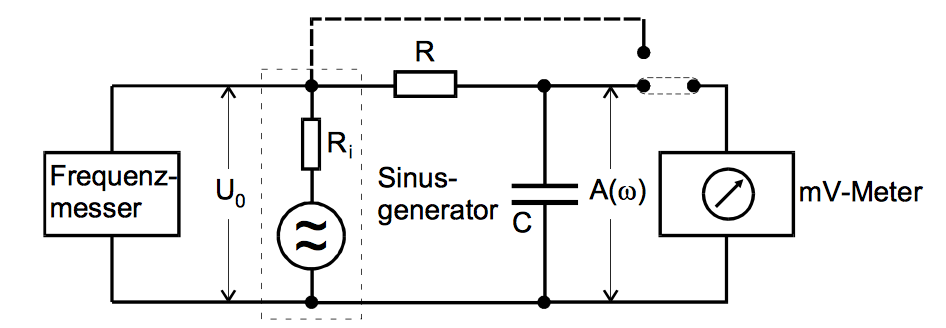
\includegraphics[width=300pt]{data/4b_schaltung.png}
  \caption{Schaltung zur Bestimmung der Zeitkonstante eines RC-Gliedes über die Messung
  der Amplitude in Abhängigkeit von der Frequenz \cite{Versuchsanleitung}}
  \label{fig:Schaltung_4b}
\end{figure}

Bei der Bestimmung der Zeitkonstanten des RC-Gliedes über die Messung der Phasenverschiebung
von der Generatorspannung $U_{\text{G}}$ und der Spannung $U_{\text{C}}$ am Kondensator
muss zunächst eine vom Multimeter erzeugte Spannung an das RC-Glied angelegt werden.
Auf dem Oszilloskop werden beide Spannungen angezeigt. Dies lässt sich mit der in \ref{fig:Schaltung_4c}
gezeigten Schaltung realisieren. Für die gleichen Frequenzen wie bei der vorherigen
Methode wird der zeitliche Unterschied $a$ der Nulldurchgänge der beiden Graphen gemäß
\ref{fig:phasenverschiebung} gemessen. Die Phasenverschiebung entspricht dann
\begin{equation}
  \phi=\frac{a}{b}2\pi\,.
\end{equation}

\begin{figure}
  \centering
  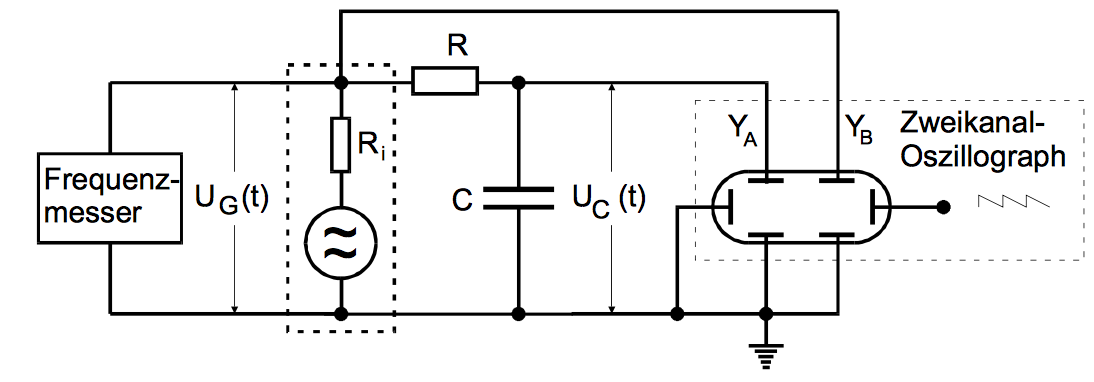
\includegraphics[width=300pt]{data/4c_schaltung.png}
  \caption{Schaltung zur Bestimmung der Zeitkonstante eines RC-Gliedes über die Messung
  der Phasenverschiebung in Abhängigkeit von der Frequenz \cite{Versuchsanleitung}}
  \label{fig:Schaltung_4c}
\end{figure}

\begin{figure}
  \centering
  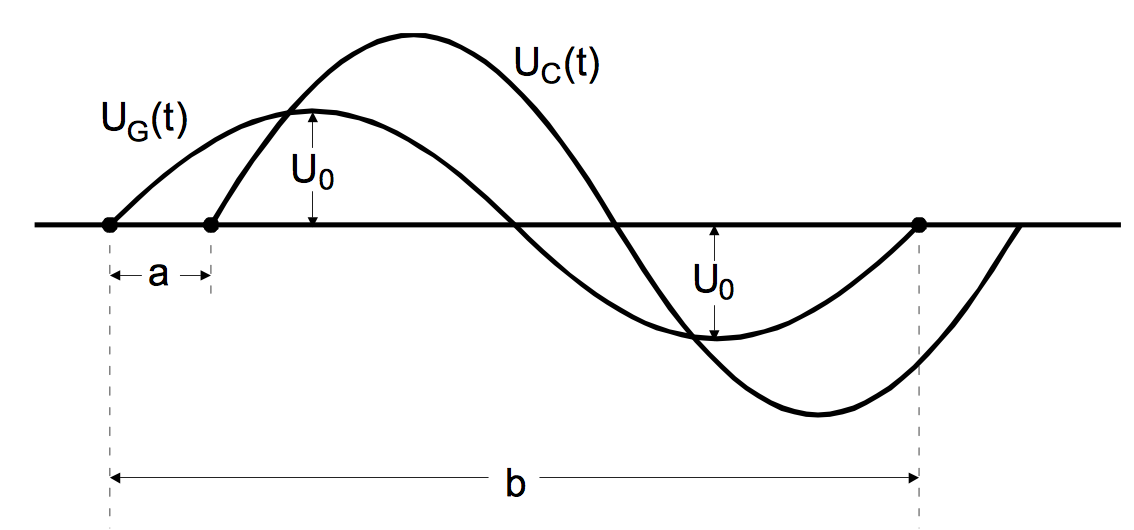
\includegraphics[width=300pt]{data/phasenverschiebung.png}
  \caption{Skizze zum Ablesen der Phasenverschiebung \cite{Versuchsanleitung}}
  \label{fig:phasenverschiebung}
\end{figure}

Um zu zeigen, dass das RC-Glied auch als Integrator dienen kann, muss eine sehr hohe
Frequenz am Multimeter einstestellt werden. Die Spannung des Multimeters wird an das
RC-Glied angelegt. Auf dem Oszilloskop werden die Spannung $U_{\text{G}}$ des Multimeters und des
die am Kondensator abgegriffene Spannung $U_{\text{C}}$ dargestellt. Es kann erneut die Schaltung
aus \ref{fig:Schaltung_4c} verwendet werden. Es sollen drei verschiedene
Spannungsmuster dargestellt werden: Sinusspannung, Sägezahnspannung und Rechteckspannung.
Für jede Spannung wird ein Bild der Graphen erstellt.
